\section{Shot Prediction}\label{ch:shot}

This chapter describes the process of retrieving the proper in-game flight parameters. Prior to Version 2018 the trajectory calculation was estimated with \class{ab.planner.TrajectoryPlanner}. However, there are a couple of issues with this approach. First, the calculation is limited to the red bird and only up to an angle of \ang{75}. Further, the launch angle is clustered into \ang{5} steps which makes it somewhat inaccurate in that window. Finally, the calculation is not a pure mathematical equation but refined with a \texttt{for} loop and small delta changes.

\paragraph{What we achieved:} The presented solution reduces the iteration count from \SI{100}{iterations} down to \numrange{3}{5}. The trajectory estimation now considers all bird types and goes well beyond the \ang{75} mark nearly up to \ang{90}, allowing very high shots in the near slingshot area (and figuring out the original version is incorrect for black and white birds for angles between \SIrange{69}{75}{\degree}). Moreover, we implemented an estimation for the yellow bird in the last project phase which isn't used at the moment but ready to enable it (there are a couple of more options to estimate the yellow bird trajectory, see \ref{ch:shot:yellowbird}).




\subsection{Slingshot Detection}
Rather by lack of knowledge (missing Chrome 2D drawings flag) we implemented a different slingshot detection mechanism which performs better in most cases. Coming with its own faults, see Edge Cases.

\begin{description}
	\item[The original detection](\class{ab.vision.VisionMBR:findSlingshotMBR()})\\
	Uses a Flood fill algorithm to group points of similar color into chunks of visual features. The RGB color space of the screenshot is quantized to a single number (representing a 3-Bit color). Then, the Flood fill checks for \num{9} pre-defined color values in that color space. A visual feature is only returned if the height is greater than the width (and some other properties).
	
	\item[The new detection](\class{features.VisionSling})\\
	Similar to the original method, a seed fill algorithm is used to group visual features. Contrary the screenshot is first converted into the HSV color space. All pixel with a hue value below a threshold of \num{18} (very dark objects) are clustered. Small clusters with less than \SI{60}{px} or with a fill ratio greater than \SI{40}{\%} will be filtered out.
	
	In most cases this leaves us with one or two visual features. Then a second thresholding is preformed only on these remaining regions. This time keeping px with hue \num{<60}, point \num{>130} and fill ratio \SI{<60}{\%}. The first iteration only gets the leftmost slingshot outline (b) whereas the second iteration returns the complete slingshot (c). The parameters are not properly tweaked, except for the hue value.
	
	\begin{center}
	a) 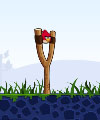
\includegraphics[height=3cm]{img/sling_detection_1}
	b) 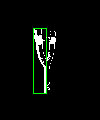
\includegraphics[height=3cm]{img/sling_detection_2}
	c) 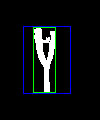
\includegraphics[height=3cm]{img/sling_detection_3}
	\end{center}
	
	\item[Edge cases] Before changing any parameters make sure to test it thoroughly with slingshots standing on various grounds (grass, wooden structure, hills, above air, below ground) and different birds in the sling (especially black and white birds). Another detection issue is high up in the clouds. One of the previous competition levels had the sling in the upper half of the screen.

\end{description}




\subsection{General Estimation Difficulties}

The open question is, can we calculate a perfect parabola prediction of the birds trajectory. Every scene is different, with a different scene scale and probably different flight characteristics per bird. How can we estimate the correct scale if the whole visual detection is prone to error? At least, we need a way to evaluate the trajectory after the first shot.


\subsubsection{Scene Scale and Magic Scaling Number}

Let's assume we already have a functioning trajectory estimation, but that estimation is limited to a fixed screen size. We need to transform the given calculations to a scene scale other then the optimized solution. We achieve that by computing a normalized scene. For this purpose we use the pixel scale of the already detected slingshot. In \class{database.Slingshot:getSceneScale()} the dimensions of the sling (width $+$ height) are combined into a single number. That number is what we simply refer to as \textbf{scene scale} (usually between \SIrange{55}{80}{px}).


Another scale, not to be confused with, is the \textbf{magic scaling number}. It can't be measured with the visual feature extraction. In fact the area defining the scene scale can be arbitrary. Looking at a level \texttt{.json} file we see two camera viewports `Slingshot' and `Castle'. By manipulating any or both viewports we identify that the scene scale is calculated somehow between these two. We don't know how the scale is calculated and more important even if we would, we couldn't access this information during runtime. This is where the \textit{magic scaling number} comes into play. Every time a shot is made, the predicted trajectory is compared against the actual flight parabola of the bird. Applying incremental updates to this magic number until eventually reaching the correct value. This number is usually somewhere between \numrange{0.95}{1.03}, stored in \class{meta.Level:scalingFactor} and reused upon revisiting the same level.


\subsubsection{Parabola Evaluation (after shot)}

As mentioned before we need to evaluate and compare the shot against our initial prediction. Luckily the game itself already draws the shot trajectory with small, white pixel clouds. Again, the original implementation in \class{ab.vision.VisionMBR:findTrajPoints()} uses quantized colors (\num{3} in this case) and Flood fill to extract the trajectory points (only taking pixel sets with max $5\times5$ px).

Our improved version \class{shot.VisionTraj} is not only extendable but also more accurate. Our version detects more clouds and at the same time includes less outliers. Furthermore the original version just took the center point of the pixel blobs bounding box. Our version computes the average point (or center of mass) under all contained points (the differences are noticeable). Finally, our method allows to split the trajectory point into a set before the tap and a set after the tap. Given that, we can utilize an autonomous shot evaluation for all bird types. Not only the default behavior but also their special capabilities and the resulting trajectory changes.

What's important to mention here is the process of filtering out outliers. First the point search is initialized at the trajectories pivot point (or at the tap point if searching for the special capability trajectory). Since we know the initial launch angle (or impact angle at tap time) we use this direction as starting direction. The next point on the trajectory (the next cloud) has to be within near distance. Also, the angle delta between the next and the previous point cannot change abruptly. From point to point the angle changes are subtle (\ang{+-23}).


\subsubsection{Launch Angle}\label{ch:shot:launchAngle}

An issue which took us quite some time to figure out, was the strange behavior of the original \class{ab.planner.TrajectoryPlanner}. Why is there even an attribute to adjust the launch angle by a small fraction (\numrange{0.025}{0.063}). Also why is this change not constant but depends on the launch angle itself. Our first guess was to rewrite the estimation completely and hope this adjustment will be gone for good. 
However, during testing even shooting with a fixed degree of \ang{45} will result in a shot that is not equivalent to the \ang{45}-shot. Even though the sent coordinates are $1000\times1000$ \si{px} away from the slingshot and the angle inaccuracy is neglectable. Turns out the game is doing some weird shit. As a consequence, we have to adjust each launch angle between shot estimation and shot execution. % lets see if this phrase will make it to the final document

The original implementation used this changeAngle multiple times throughout the estimation, whereas our version does one conversion at the end. As mentioned in the chapter introduction the original version relies on a \texttt{for} loop, whereas our version refines the angle with a recursive call. Most of the time the \num{2}. or \num{3}. iteration is already accurate up to \num{1e-5}.

But an other issue came up which is not present in the original implementation. Only because the original version has not the capability to do so. Our version has for each bird two equations. One for very-high-shots \ang{>75} and one equation for angles below \ang{75}. The very-high-shot equation is very steep so the recursive approach isn't suitable. We have to handle this case separately (see \class{shot.ShotHelper:estimateLaunchPoint()}). Furthermore, shots directly in the area where the two equations collide are probably estimated wrong (if starting with the wrong equation). Here, we have to find a better way to use both equations simultaneously.




\subsection{Class: ParabolaTester}\label{ch:shot:tester}

The \class{tester.ParabolaTester} class is the starting point for rapid prototyping and testing of new trajectory calculations. It provides a controlled environment with fixed, known slingshot dimensions and the corresponding pivot point. The mathematical equations are optimized for this specific scene scale. All needed resources are located in \source{/doc/parabolaEvaluation}.


\subsubsection{General procedure}

\begin{enumerate}
	\item To setup the environment load the \num{6} levels (\source{Level1-1.json}, etc.) into your game and change the boolean flag to \texttt{true} in \class{main.BamBird:main()}

	\item Run \class{ParabolaTester} and record raw data in \texttt{.csv} files in the root directory (all results are in the afore mentioned \source{/doc} directory).

	\item The raw file is then processed with the python script (\source{run.py}) into a readable format that is copy'n'paste accepted by Grapher (a macOS application).\\
	\textbf{Note:} If you want to omit this step, make sure you apply the same column calculations.

	\item In Grapher (or your application of choice) import the data and manually remove visible outliers (fig. \ref{img:shot:grapher}). Split the point set into separate groups with distinct features (e.g. everywhere where data points differ). Perform a curve fitting on all sets separately (Grapher: Select point set $\rightarrow$ Interpolation $\rightarrow$ Polynomial, Order 3).
	
	As seen in section \ref{ch:shot:launchAngle} we need an equation for the launch angle change and another equation for the velocity. Both equations take the launch angle (in radians) as input and output the corrected launch angle as well as the velocity needed to predict the parabola. Finally, we have to find the intersection point between the high shot and the low shot equation (Grapher: Select both equations $\rightarrow$ Menu Equation $\rightarrow$ Find Intersection).
	
	\item Save the results (Grapher \texttt{.gcx} file \& \source{fnGraphs.txt}) and export the data to Java.
\end{enumerate}


\begin{figure}
	\centering
	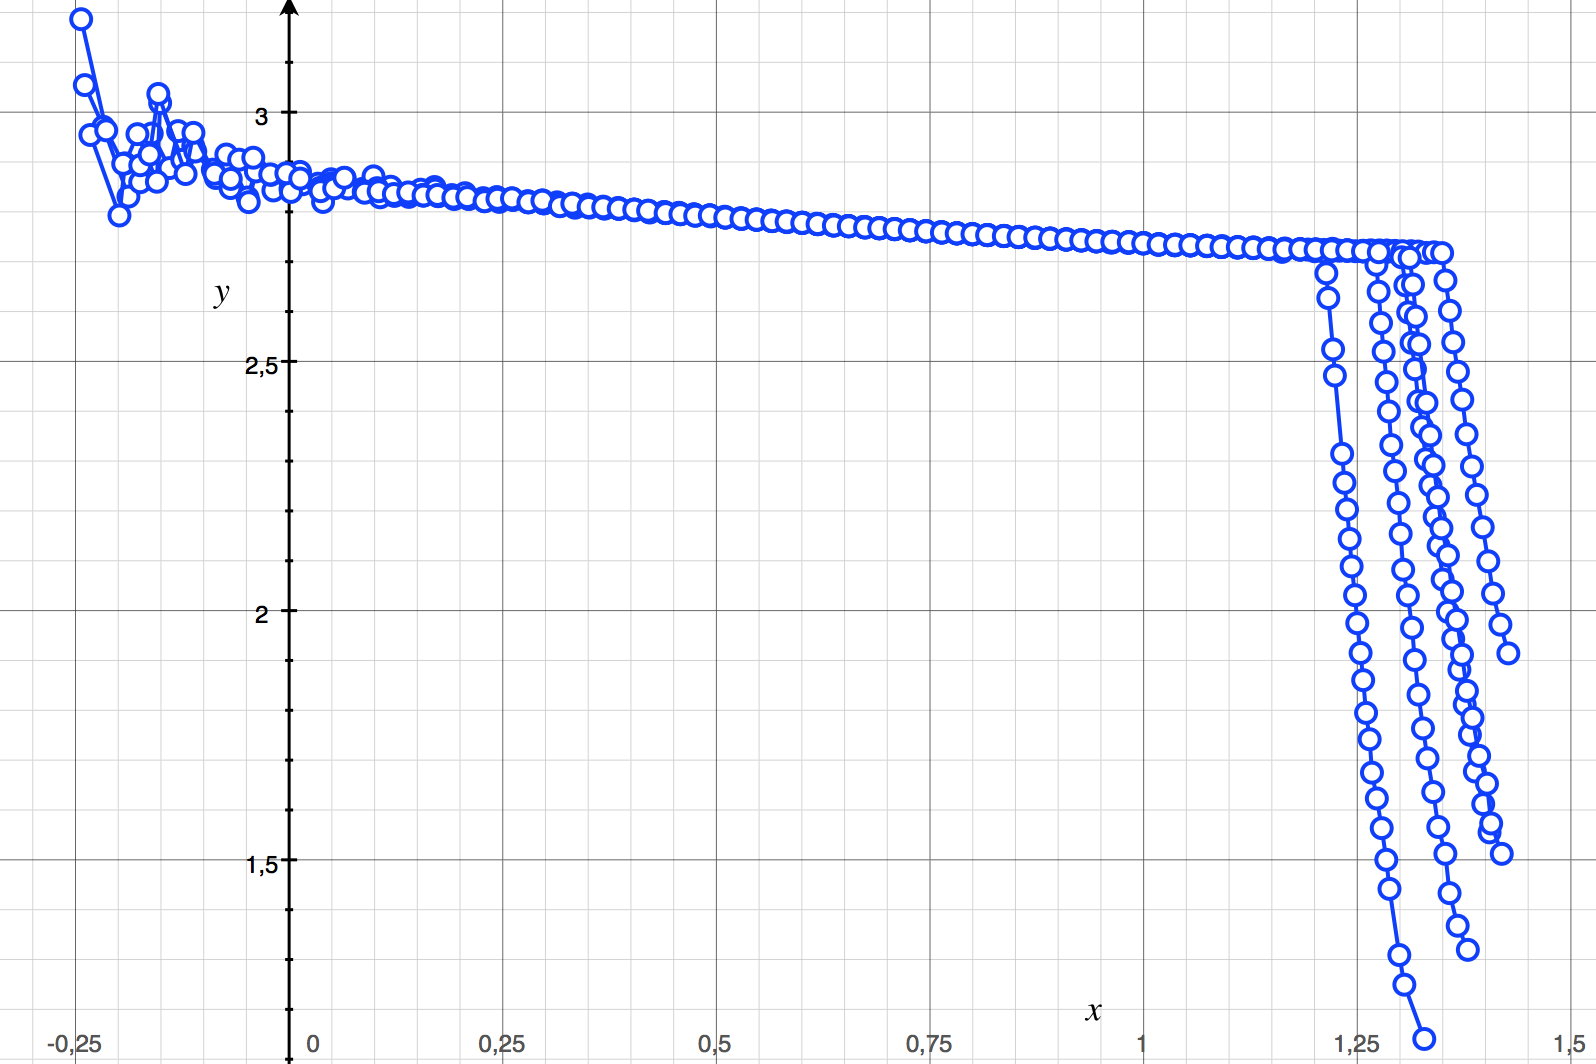
\includegraphics[width=12cm]{img/shotVelocity}\\
	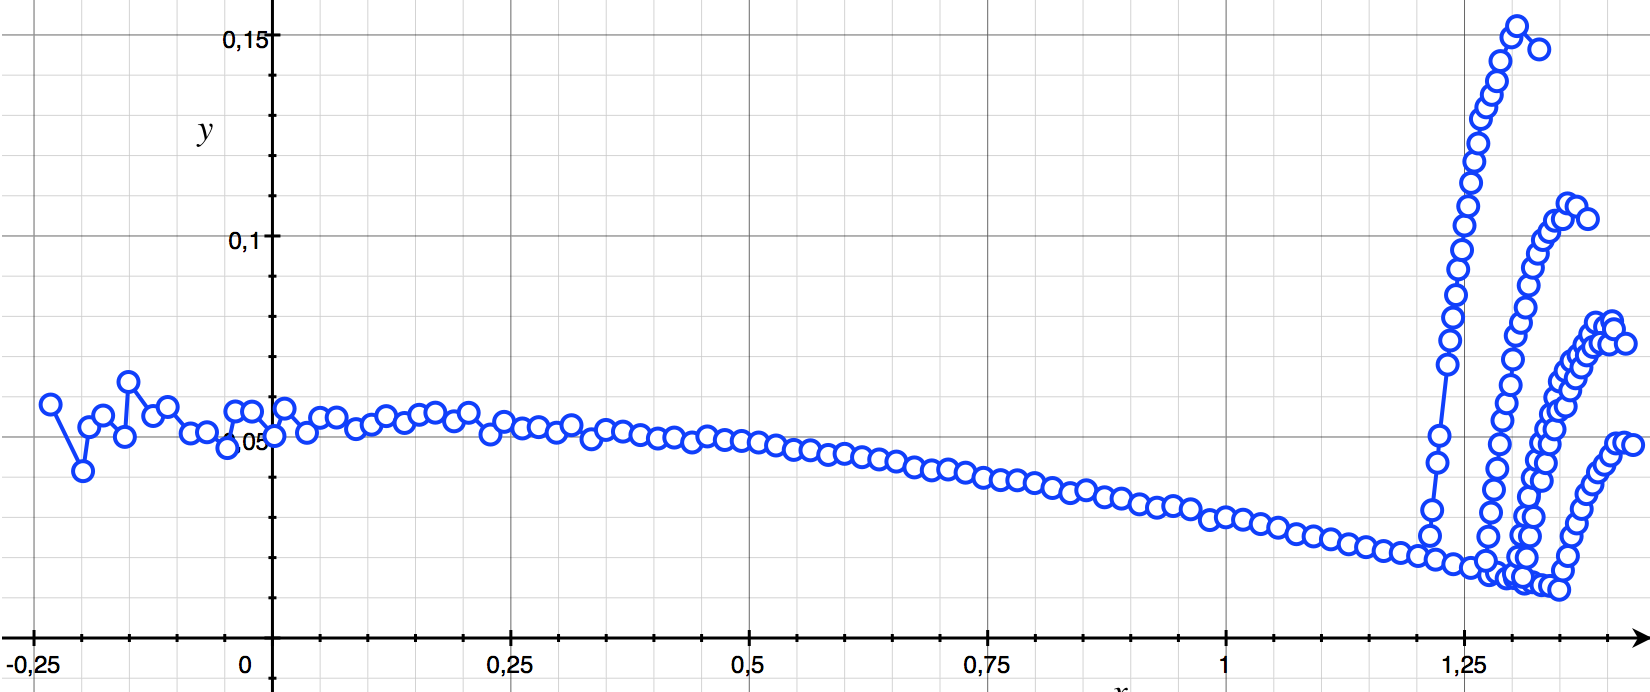
\includegraphics[width=12cm]{img/shotAngle}
	\caption{Raw data points for launch velocity (top) and adjusting angle (bottom) for all birds. X-axis: launch angle, Y-axis: velocity / change delta}
	\label{img:shot:grapher}
\end{figure}



\subsubsection{Different Testing Methods}

\begin{description}
	\item[\class{createShotEvaluationForAllBirds()}]$~$\\
	For all bird type try all shots between \SIrange{0}{86}{\degree}. Using \ang{1} steps until \ang{74} and \ang{0.5} beyond. Numerous tests have shown, that the low shots (red bird \ang{<74}, white bird \ang{<69}) are identical for all bird types. Therefore, this test will evaluate this range only once for the red bird. The very-high-shot ranges are evaluated for all birds nonetheless. The whole run takes roughly \SI{1}{\hour}.
	
	\item[\class{findAccuratePivotPoint(ABType)}]$~$\\
	Loads the level of the corresponding bird type and shoots at \num{4} different angles with \ang{10} spacing between. Each pair of two shots has an intersection somewhere in the slingshot area. This point is calculated and print to standard output (no file output!). Repeating this for all bird types will yield a (hopefully) accurate pivot point. All tests take \SI{5}{\minute}.
	
	\item[\class{findYellowBirdEstimation()}]$~$\\
	Similar to all birds evaluation the whole spectrum of the yellow bird special capability is covered. Testing impact angles (angle at tap point) from \ang{-65} to \ang{23}. Trying to shoot with different launch angles to add some variation. The result is somewhat unpredictable since it relies on a proper tap time estimation. However, the game server isn't very precise when it comes to tap time \dots This test alone takes \SI{38}{\minute}.
	
	\item[\class{shootRandomPoints()}]$~$\\
	Quick \num{9}-shot evaluation if the current equation parameter are accurate. Enable visual output (\class{DBG.enableDebug()}) to check if predicted parabola is identical to actual parabola.
	
	\item[\class{shootRandomPointsYellowTap()}]$~$\\
	Same as the test above but for yellow birds with automatic tap time estimation. \SI{1}{\minute}.
	
	\item[\class{shootYellowNear()}]$~$\\
	Does nothing yet. The idea was to predict a target point with normal trajectory estimation. Then adjust this given parabola slightly to the left to accurately hit the target even with yellow bird tap. With current implementation the yellow bird will always overshoot. 
	
	\textbf{Note:} This has to work independently of target position (even with impact angle \ang{>0})!
\end{description}




\subsection{Special Bird Estimation}

The parabola evaluation in section \ref{ch:shot:tester} has shed light onto boundaries of the original trajectory estimation. Because of the different bird sizes, very high angles will be cut at different angles for all birds (white: \ang{69} vs. blue: \ang{77}). Before version 2018 the special capabilities of different bird types were only considered rudimentary (blue: shoot ice, black: destroy as much as possible, yellow: go for wood). We are constantly moving closer to a full-featured tap-time prediction for all birds. Below is the current state of the software as well as some observations and suggestions on implementing the remaining estimations.


\subsubsection{Yellow Bird}\label{ch:shot:yellowbird}

We currently support only one type of yellow bird estimation. For a given target and a \textbf{fixed launch angle} we can estimate the tap point (\class{shot.ShotHelper:predictYellowBirdTapPoint()}). This approach will fail if the target can't be reached with the predefined launch angle. The tap-to-target trajectory is estimated as a straight line and refined successively (max \num{20} iterations) with the actual yellow bird equation.

Another type of yellow bird estimation (not implemented yet) is found by \textbf{refining the original parabola estimation}. The one calculated if no tap is happening (or `red bird estimation'). We already have a parabola estimation for the target without tap time. If the yellow bird is tapped (special capability activated) the bird will definitely overshoot and miss the target. On the other hand, we want to use the stronger shot gained from a tap. Therefore, we have to adjust the parabola to hit the target particularly with tap time. For near targets the launch angle needs to be adjusted more steep, whereas for far away targets the launch angle has to be lowered.

The third type for yellow bird estimation is \textbf{fixed impact angle} (not implemented yet). Sometimes we want to hit the target with a precise angle. For example, when an indestructable hill is blocking all other shot options (aka funnel). Although we don't see this type as very important, it could improve our performance in some rare cases tremendously.


\subsubsection{White Bird}

The estimation for white birds is rather simple. Start from the target you want to hit and go up in a straight line until you find a point that is hittable with normal estimation. This assures an egg-bomb will have a free fall to hit the target. Although currently implemented in Prolog, a Java implementation is missing. Depending on the future development, all estimations will be handled either in Prolog or Java.


\subsubsection{Black Bird}

The strategy for black birds is handled completely in Prolog. From the Java perspective we will always tap to make the bird explode. Prolog decides where the highest impact can be reached (and avoids black bird traps). We can still improve the prediction by allowing timed tapping. Sometimes its better to tap as early as possible, other times to wait until the bird explodes on its own. Pigs can be killed through hills if timed correctly.


\subsubsection{Blue Bird}

Although there is no blue bird estimation yet, a couple of observations: The middle path of the blue bird split will always stay unchanged. The other two paths split at the same angle in both directions. Also, since the middle path is unchanged, gives us a clue that the velocity doesn't change after the tap. Which in return means, that only the angle of the trajectory is changed in mid-air.

One option is to extend \class{tester.ParabolaTester} with an additional blue bird test. This includes clustering of the points after the tap into three groups (low, mid, high). The mid path can be found easily by extending the parabola before the tap. All other points lay either above or below this parabola. Points near the tap point and very high shots will distort the results (High shot: because the low split will project into the part before the tap and therein filtered out 'cause of abrupt angle change).

The second option is to manually try a few angles. Write a simple random blue bird tap shooter and experiment with fixed angles for both (high and low) splits. The velocity should be the same as the velocity at the tap point. Using the impact angle at tap point as base direction. Here again a piece of advice, the tap time isn't always accurate. A few bad runs don't necessarily mean the parameters are bad.




\subsection{Non-Working Alternatives}\label{ch:shot:fails}

This chapter summarizes all approaches we have tried but didn't led to success. Testing any further in that direction doesn't make sense, there are other areas to improvement.

We put a lot of effort into finding a solution that doesn't rely on adjusting the launch angle for each shot. One thing that doesn't affect the flight path is \textbf{gravity}. Changing the gravity for different birds is the same as having a unique equation per bird. Nonetheless all calculations in \class{helper.ParabolaMath} respect the gravity constant. Though the static variable \texttt{\_g} is fixed to \num{1.0} (compiler optimization will ignore the unnecessary calculation anyway).

Also searching for a solution that better reflects the slingshots \textbf{pivot point} is wasted time. The current solution is accurate up to \num{4.5e-3} on relative values (\numrange{0.0}{1.0}, value $\times$ sling width). Instead of tweaking the parameters in \class{database.Slingshot:calculatePivot()} (generated by \class{tester.ParabolaTester:findAccuratePivotPoint()}), we need to optimize the detection of the slingshot. If the detected rectangle is faulty, the resulting pivot point will vary heavily. We can't be sure that neither the slings height, nor the slings width will be detected correctly. Currently, the height is ignored because in many test levels the sling was lowered too deep into the ground. A size independent slingshot detection isn't feasible yet, since the scene scale relies on that measure too.


\textbf{One calculation for all bird types} would be the preferable solution, especially for high shots. But experimenting with various settings, there is no rule between the birds size and the very-high-shot change angle. Of course there is, but non that is eminent and can be used with the available information. Theoretically the bird size should influence the high angle cutoff exclusively. However, the real bird sizes (\class{database.ScreenScale}) dont't even have the same ratio as the in-game bird sizes. In theory, the high angle cutoff should be a straight line, instead the line is slightly bend (compare fig. \ref{img:shot:grapher} top).

